\chapter{Conclusions and future work}
\label{conclusions}

%% Built an ideal platform to do a lot of things
%% Move to 3d, staggered, non-proprietary environment
%% Revert to using physically motivated strain energy functions, and
%% base this for instance on experiments on whether temperature
%% affects the mechanics in the ``appropriate way.''
%% Use the combinations (porous, viscoelastic solid with viscous fluid
%% perfusing, etc.) to nail down biphasic mechanics.
%% Can be specialised to other things in a fairly straightforward
%% manner, such as tyre-filling.
%% Flesh out the stress-dependent growth laws and tie more intimately
%% with experiment. Healing, and cancer.
%% Incorporate more advanced biochemistry within the overarching
%% framework.
%% hyperelasticity. Mention others, such as the complicated one used
%% earlier and elastica, when close comparisons with experiment are
%% required.



%% \todo{\begin{itemize}
%%   \item Work on this chapter in the end, after Chapter 1.
%%   \item Summarise what was achieved, and how else it could be used. The
%%     length of this chapter is probably going to be the least.
%%   \item Point back to modern literature and show how this differs, why
%%     it's useful, and why it's cool.
%% \end{itemize}}

\section{Discussion and conclusions}
\label{discussion}

A general framework for growth of biological tissue has been
presented in this paper. While simplified models were used for
source terms, $(\Pi^\iota)$, they can be formulated on the basis
of the kinetics of chemical reactions in order to develop more
realistic growth laws. This approach, we believe, is fundamental
to a proper treatment of mass transport in tissue. Results are
obtained that differ fundamentally from the classical setting of
continuum mechanics. Most notable among these differences are the
mass fluxes driven by gradients in stress, strain, energy and
entropy, in addition to body force and inertia. Importantly,
though our treatment differs from classical mixture theory, the
two are fully consistent as established at several points in this
paper. The balance laws in Section \ref{sect2} and \ref{sect3}
introduce a degree of coupling between the phenomena of mass
transport and mechanics. This is visible most transparently in the
balance of linear momentum (\ref{ballinmomrefI}) that includes
mass fluxes, $\bM^\iota$. The balance of mass, described by
Equations (\ref{massballocA}) and (\ref{massballocI}), is also
dependent upon the mechanics as the discussion in Section
\ref{sect5.1} makes clear. Notably, this ensures
mechanics-mediated mass transport even with a mass source that is
independent of strain/stress, as the discussion at the end of
Section \ref{sect5.3} establishes. The discussion in Sections
\ref{sect5.1}--\ref{sect5.3} provides many insights into the
nature of this coupling. The mechanics problem also has a
constitutive dependence upon mass concentration, via
(\ref{stress-constrelI}) and the fact that the growth deformation
gradient tensor, $\bF^{\mathrm{g}^\iota}$ is determined by the
concentration. The viscoelastic nature of the composite tissue
would emerge naturally from a model incorporating a hyperelastic
solid and viscous fluid.

We have formally allowed all species to be load bearing and
develop a stress. At the scales that are of interest in a tissue,
the only relevant load bearing species are the solid and fluid
phases. Nevertheless, inasmuch as a transported species such as a
nutrient has a molecular structure that can be subject to loads at
the scale of pico-newtons, it is not inconsistent to speak of the
partial stress of this species. Since the constitutive relation
(\ref{stress-constrelI}) indicates that the partial stresses are
scaled by concentrations, the contribution to total stress from
any species besides the solid and fluid phases will be negligible.

We have chosen to leave remodelling out of our formulation in this
communication, to focus upon the above issues. Remodelling
includes any evolution in properties, state of stress, material
symmetry, volume or shape brought about by microstructural
changes. In the development of biological tissue, growth and
remodelling occur simultaneously. As density changes due to
growth, the material also remodels by microstructural evolution
within the neighborhood of each point. A rigorous treatment of
this phenomenon has been presented in the continuum mechanical
setting in a companion paper \citep{remodelpaper}.

\section{Suggestions for future work}
\label{future-work}

In this paper, we have discussed a number of enhancements to our
original growth formulation presented in \citet{growthpaper}. That
formulation has served as a platform for posing a very wide range of
questions on the biophysics of growth. Some issues, such as
saturation, incompressibility of the fluid species and its influence
upon the tissue response, and the roles of biochemical and strain
energy-dependent source terms are specific to soft biological
tissues. We note, however, that other issues are also applicable to a
number of systems with a porous solid, transported fluid and reacting
solutes. Included in these are issues of current versus reference
configurations for mass transport, swelling, Fickean diffusion, fluid
response in compression and tension, cavitation and the strength of
solid-fluid coupling..

These issues have been resolved using arguments posed easily in the
framework derived in Chapters~\ref{lagrangian-perspective} and
\ref{eulerian-perspective}. The 
interactions engendered 
in the coupled reaction-trans\-port-mechanics system are complex, as
borne out by the numerical examples in
Chapter~\ref{numerical-simulations-1}. We are currently examining
combinations of sources defined in Section~\ref{nature-of-sources}, and aim to
calibrate our choices from tendon growth experiments. The treatment of
these issues has led to a formulation more suited to the biophysics of
growing soft tissue, making progress toward our broader goal of
applying it to the study of wound healing, pathological hypertrophy
and atrophy, as well as a study of drug efficacy and interaction.

 It is therefore somewhat less motivated and more
questionable. Clearly, a rigorous analysis or numerical comparisons of
all three models: upper bound, lower bound and direct solution of
individual solid-fluid momentum balances, must be carried out to
conclusively demonstrate this.

\subsubsection{Non-linear viscoelasticity}
\label{non-linear-viscoelasticity}

\begin{figure}[!hptb]
\centering
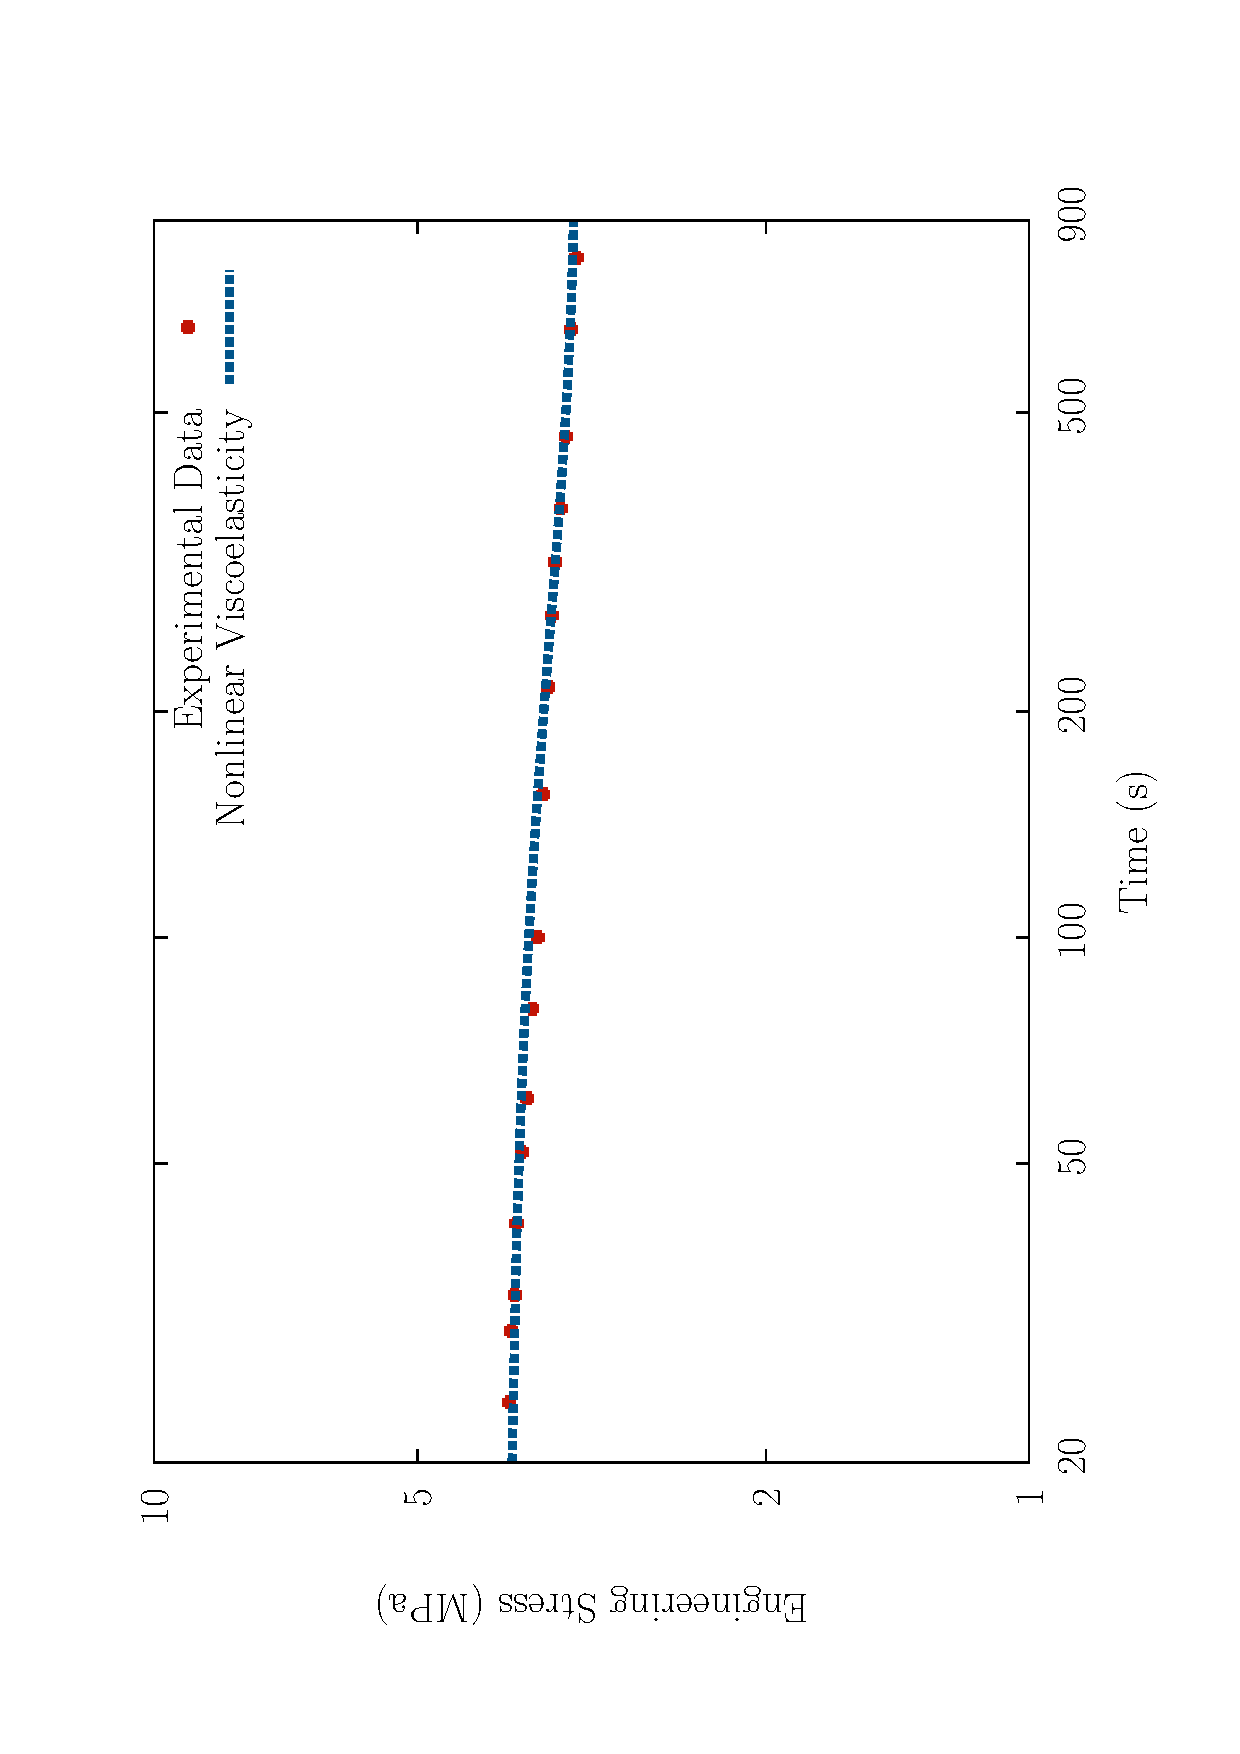
\includegraphics[width=0.6\textwidth,angle=270]{images/examples/%
eulerian/nonlinear-viscoelasticity/provenzano-data-comparison}
\caption{The non-linear time constants fit to experiment.} 
\label{provenzano-data-fit}
\end{figure}

\begin{figure}[!hptb]
\centering
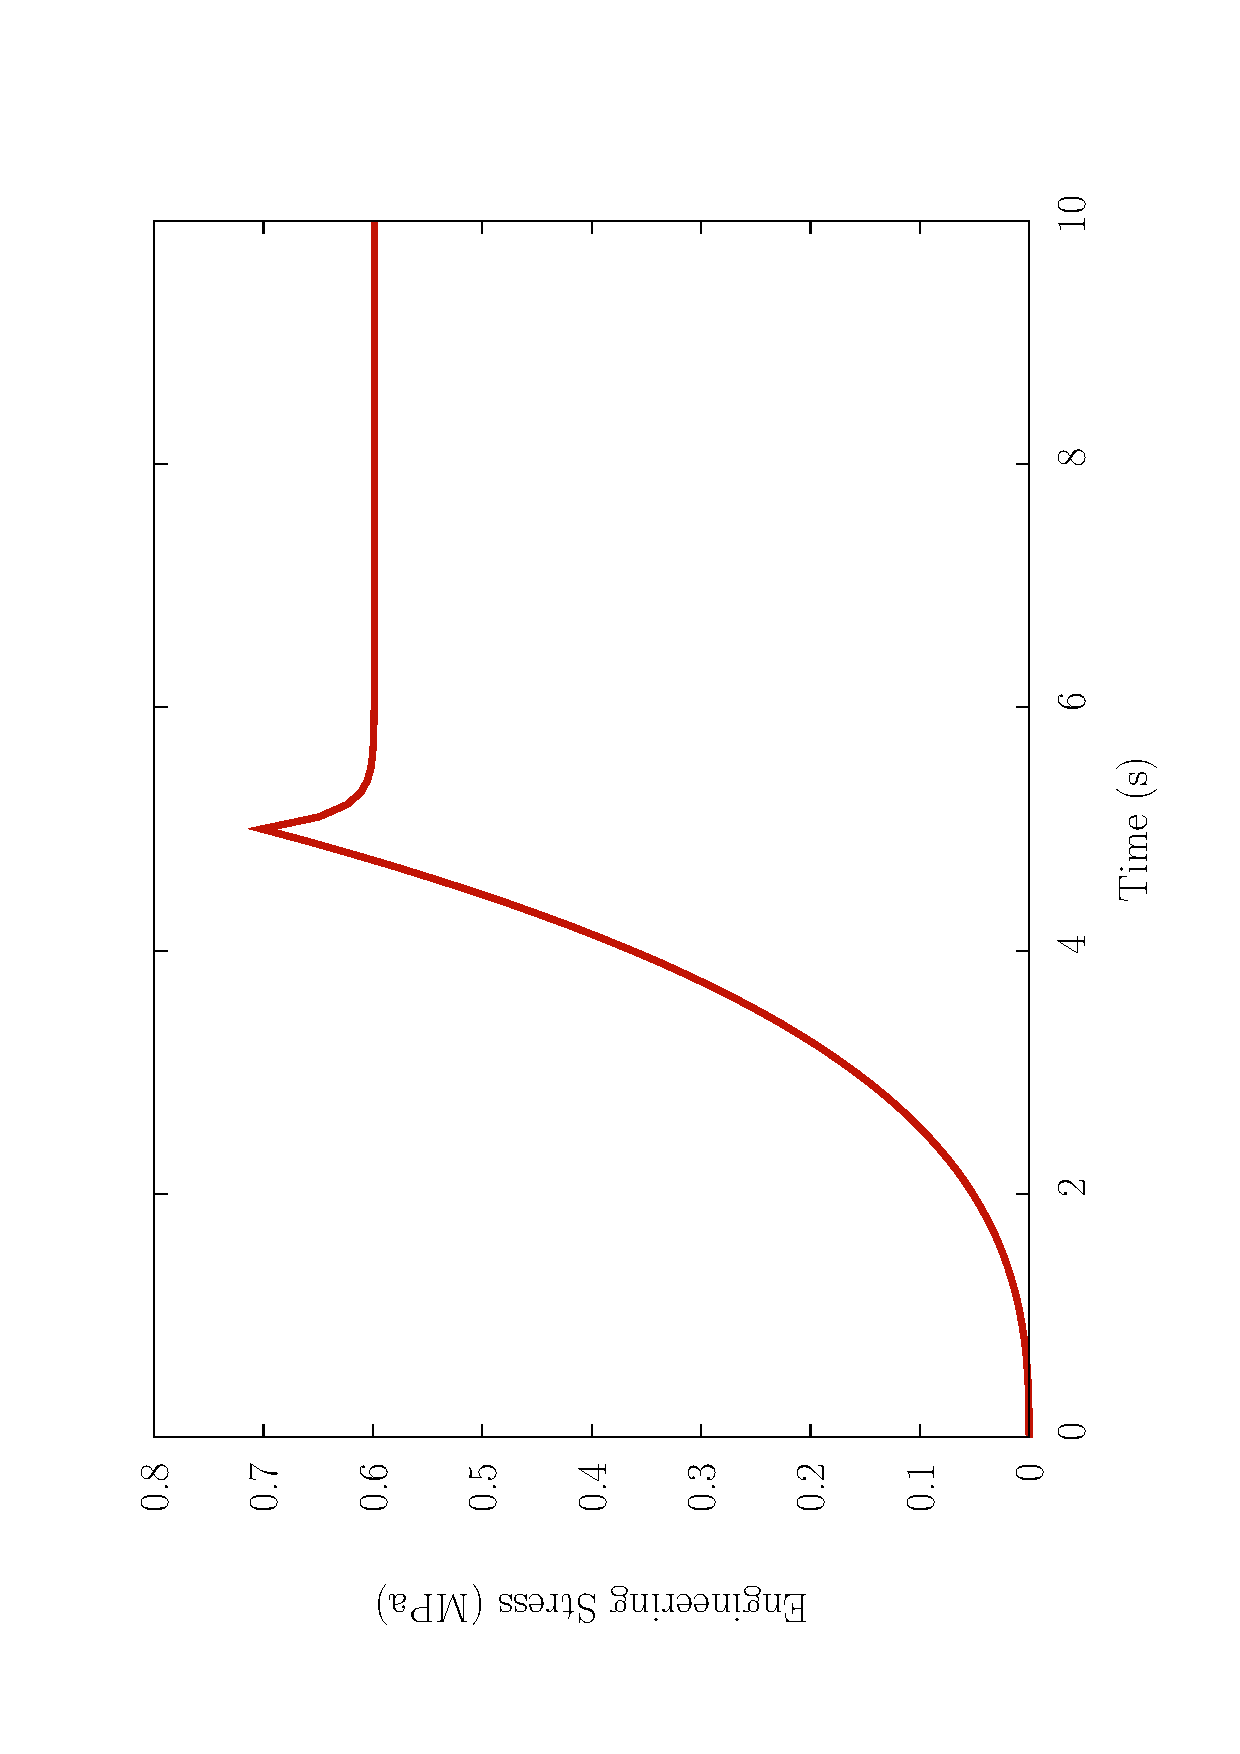
\includegraphics[width=0.6\textwidth,angle=270]{images/examples/%
eulerian/nonlinear-viscoelasticity/nonlinear-viscoelasticity-stress-relaxation}
\caption{Stress relaxation under nonlinear viscoelasticity.}
\label{nonlinear-viscoelasticity-stress-relaxation}
\end{figure}

% Perhaps also show flow fields of a viscous fluid. The emphasis here
% is on combinations for studying aspects of mechanics, then onto
% growth.

%%The calculations presented in 
%% All the calculations presented in Section~\ref{} have used the same
%% material constants resulting in the same general shape and
%% stress-strain ranges of the results. This can be, and has been,
%% tweaked to fit other sorts of curves changing both ranges and shapes
%% by tweaking the Mooney-Rivlin constants.

%

% Local Variables:
% TeX-master: "thesis"
% mode: latex
% mode: flyspell
% End:
